\section{Statistical Analysis of Surface Features}
\label{sec:statistical-validation}

Section~\ref{subsec:lexical-separability} requires the sample set to be balanced across sub-agents in writing style, punctuation, and sentence pattern, not only in vocabulary. Without that balance, a text-only classifier could route a request by a stylistic marker instead of by what the request asks. This section reports an analysis of variance (ANOVA) that tests whether the dataset meets that requirement, over measurable \emph{surface features} of the request text, properties that define how a request is written, such as its length or its punctuation, computed directly from the characters and words of the request text.

\subsection{Design Factors}
\label{subsec:design-factors}

Every test in this section reads one or more of the following design factors:

\begin{itemize}
    \item \texttt{gold}: the correct sub-agent the request should be routed to.
    \item \texttt{decoy}: the sub-agent whose constraint is stated but waived, defined only when the sample carries a decoy.
    \item \texttt{difficulty}: the difficulty tier the sample was built at, \texttt{plain}, \texttt{natural}, or \texttt{adversarial} (Section~\ref{subsec:difficulty-tiers}).
    \item \texttt{pattern}: the decoy pattern used to write the adversarial pair, defined only for the \texttt{adversarial} tier (Section~\ref{subsec:difficulty-tiers}).
    \item \texttt{persona}: the writing style used to generate the request (Section~\ref{subsec:personas}).
\end{itemize}

\subsection{Sample Balance}
\label{subsec:sample-balance}

ANOVA assumes \emph{homoscedasticity}, that is, that the variance of the tested feature is the same in every group the factors define. Section~\ref{subsubsec:levene-kruskal} tests this assumption directly and finds it violated for several features. The F-test that ANOVA relies on is expected to remain robust to unequal variance when the design is balanced, that is, when every group holds the same number of samples \citep{glassConsequencesFailureMeet1972}.
This robustness is why the balance checked in this section matters beyond precision: it is also what keeps every ANOVA in this chapter valid despite the violated homoscedasticity assumption.

An unbalanced design also risks a different problem: an ANOVA can attribute variance to a factor that only occurs more often for one sub-agent, rather than to a real effect of that factor. The plan stage provides balanced samples by design (Section~\ref{subsec:pipeline-plan}), and Figure~\ref{fig:sample-balance} plots the sample counts that result.

\begin{figure}[H]
    \centering
    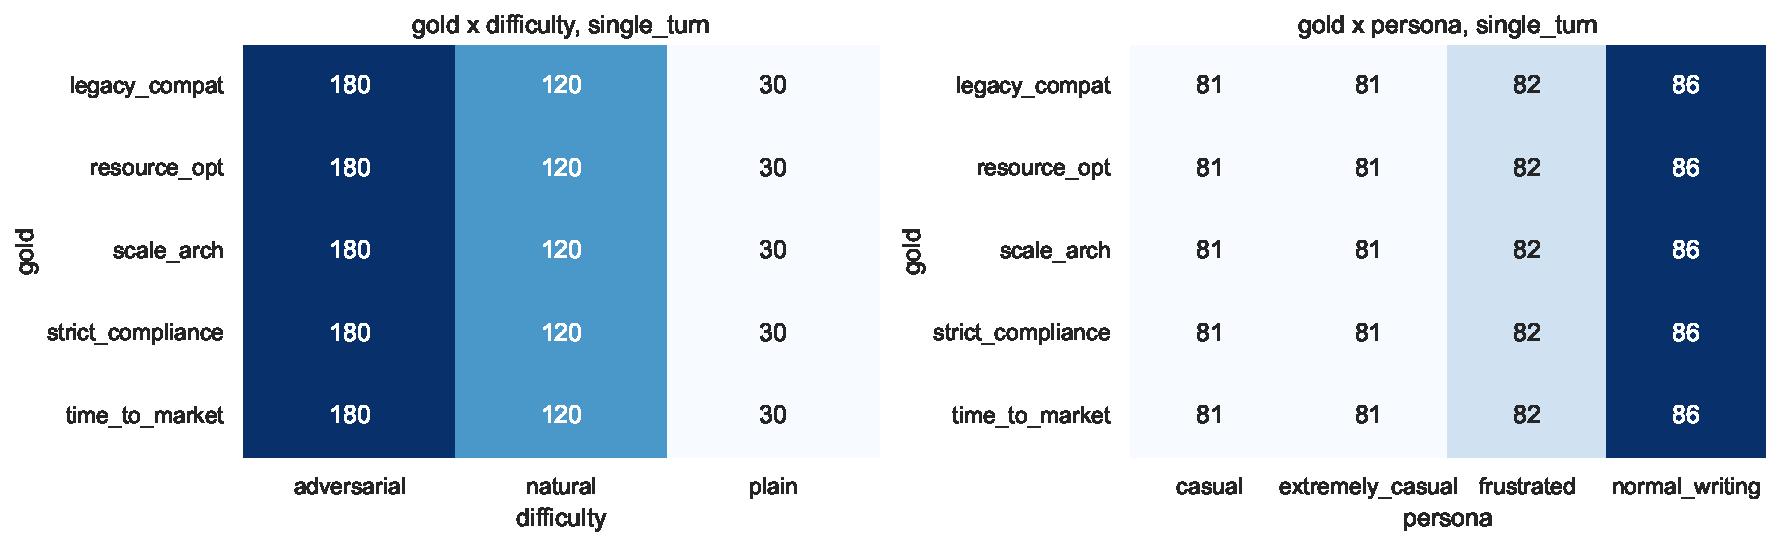
\includegraphics[width=\textwidth]{images/plots/anova/dataset_composition_single_turn.pdf}
    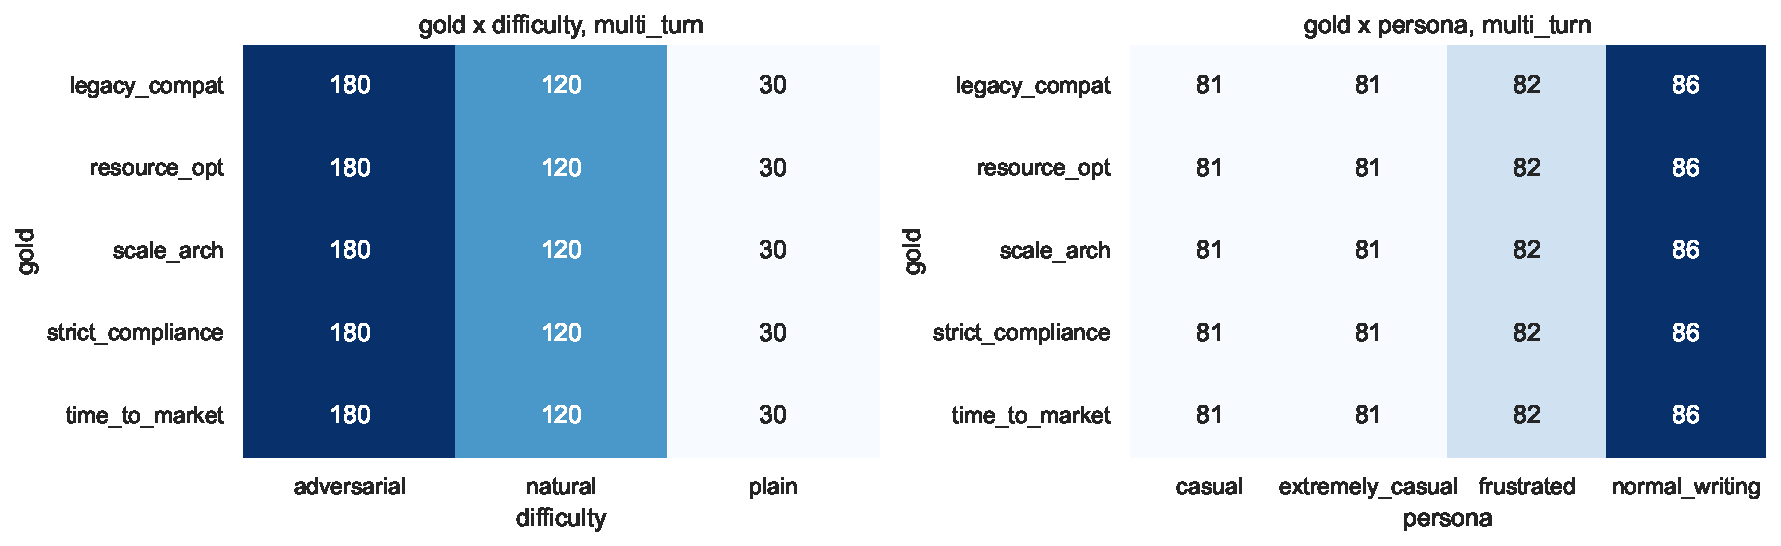
\includegraphics[width=\textwidth]{images/plots/anova/dataset_composition_multi_turn.pdf}
    \caption[Sample counts per sub-agent by tier and persona]{Sample counts per sub-agent, against difficulty tier and persona, single-turn (top) and multi-turn (bottom).}
    \label{fig:sample-balance}
\end{figure}

Figure~\ref{fig:sample-balance} cross-tabulates the correct sub-agent (\texttt{gold}) against the difficulty tier and against the persona, for the single-turn and the multi-turn dataset. Every sub-agent receives the same number of samples at every difficulty tier. Persona counts are near-equal but not identical across sub-agents, for example 81, 81, 82, and 86 samples for the four personas of a given sub-agent, because the deterministic shuffle in Section~\ref{subsec:pipeline-plan} distributes personas evenly only up to the remainder left when the sample count for a sub-agent is not a multiple of four. This gap, at most 5 samples out of about 330 per sub-agent, is negligible and does not compromise the balance that the tests in this section rely on.

\subsection{Extracted Features}
\label{subsec:surface-features}

The ANOVA in this section asks whether the correct sub-agent, \texttt{gold}, leaves a mark on the surface style of the request text, independent of its content. Section~\ref{sec:statistical-validation} requires the five sub-agents to be balanced in style: without that balance, a text-only classifier could route a request by a stylistic cue instead of by what the request asks. For each surface feature tested, the null hypothesis states that \texttt{gold} has no effect on it, that is, that the mean value of the feature is the same across the five sub-agent groups. Rejecting the null hypothesis for a feature means the sub-agent groups differ on that stylistic property.

For the ANOVA analysis, thirteen surface features are extracted from the text of each request. They are listed in Table~\ref{tab:surface-features}.

\begin{table}[H]
    \centering
    \begin{tabularx}{\textwidth}{@{}l>{\raggedright\arraybackslash}X@{}}
        \toprule
        \textbf{Feature} & \textbf{Definition} \\
        \midrule
        \texttt{n\_chars} & Number of characters \\
        \texttt{n\_words} & Number of words \\
        \texttt{n\_sentences} & Number of sentences \\
        \texttt{mean\_word\_len} & Mean word length, in characters \\
        \texttt{mean\_sent\_len} & Mean sentence length, in words \\
        \texttt{ttr} & Type-token ratio, distinct words divided by total words \\
        \texttt{pct\_upper} & Percentage of characters that are uppercase \\
        \texttt{pct\_digit} & Percentage of characters that are digits \\
        \texttt{n\_question} & Number of question marks \\
        \texttt{n\_comma} & Number of commas \\
        \texttt{long\_word\_ratio} & Percentage of words longer than seven characters \\
        \texttt{n\_units} & Count of unit and magnitude markers (\texttt{\%}, \texttt{\$}, MB, ms, req/s, and similar) \\
        \texttt{n\_number\_words} & Count of numbers written as words (\textit{eighty}, \textit{two weeks}, \textit{percent}) \\
        \bottomrule
    \end{tabularx}
    \caption[The thirteen surface features extracted from each request]{The thirteen surface features extracted from each request.}
    \label{tab:surface-features}
\end{table}

\subsection{One-Way ANOVA}
\label{subsec:anova-oneway}

For each of the thirteen surface features, a \emph{one-way ANOVA}, an ANOVA that tests one factor at a time, tests whether \texttt{gold} has an effect on that feature, for example whether the number of words in a request differs depending on which sub-agent is correct for it. Two quantities are reported for each test.

\paragraph{Effect size ($\omega^2$).} Omega squared is the percentage of the total variance in the feature explained by \texttt{gold}, corrected for the sampling noise that a simpler estimate (eta squared) would count as effect \citep{olejnikGeneralizedEtaOmega2003}. Cohen defines conventional thresholds for eta squared at 0.01 as small, 0.06 as medium, and 0.14 as large \citep{cohenStatisticalPowerAnalysis2013}; these thresholds are reused for omega squared as well.

\paragraph{Corrected significance ($p_{\text{holm}}$).} A one-way ANOVA returns a $p$-value for the null hypothesis that \texttt{gold} has no effect on a given feature. A raw $p$-value below 0.05 would count that effect as significant on its own. But thirteen tests are run at once, one per feature, and some of them are expected to fall below 0.05 purely by chance, even if \texttt{gold} has no real effect on any feature. The Holm method \citep{holmSimpleSequentiallyRejective1979} corrects for this. It raises the threshold each test must clear as more tests are run, and the corrected $p$-value is reported as $p_{\text{holm}}$. An effect counts as significant only when $p_{\text{holm}}$ stays below 0.05.

\bigskip

\begin{table}[htbp]
    \centering
    \small
    \begin{tabular}{@{}lrrrr@{}}
        \toprule
        & \multicolumn{2}{c}{\textbf{Single-turn}} & \multicolumn{2}{c}{\textbf{Multi-turn}} \\
        \textbf{Feature} & $\omega^2$ & $p_{\text{holm}}$ & $\omega^2$ & $p_{\text{holm}}$ \\
        \midrule
        \texttt{pct\_digit}        & \cellcolor{omegaMedium}0.132 & \textbf{$<$0.001} & \cellcolor{omegaMedium}0.082 & \textbf{$<$0.001} \\
        \texttt{n\_units}          & \cellcolor{omegaMedium}0.119 & \textbf{$<$0.001} & \cellcolor{omegaMedium}0.090 & \textbf{$<$0.001} \\
        \texttt{mean\_word\_len}   & \cellcolor{omegaMedium}0.063 & \textbf{$<$0.001} & \cellcolor{omegaMedium}0.075 & \textbf{$<$0.001} \\
        \texttt{long\_word\_ratio} & \cellcolor{omegaMedium}0.062 & \textbf{$<$0.001} & \cellcolor{omegaSmall}0.046  & \textbf{$<$0.001} \\
        \texttt{n\_comma}          & \cellcolor{omegaSmall}0.036  & \textbf{$<$0.001} & \cellcolor{omegaSmall}0.016  & \textbf{$<$0.001} \\
        \texttt{n\_chars}          & \cellcolor{omegaSmall}0.024  & \textbf{$<$0.001} & \cellcolor{omegaSmall}0.015  & \textbf{$<$0.001} \\
        \texttt{n\_words}          & \cellcolor{omegaSmall}0.016  & \textbf{$<$0.001} & 0.006 & \textbf{0.038} \\
        \texttt{n\_number\_words}  & \cellcolor{omegaSmall}0.015  & \textbf{$<$0.001} & \cellcolor{omegaSmall}0.011  & \textbf{0.002} \\
        \texttt{ttr}               & \cellcolor{omegaSmall}0.014  & \textbf{$<$0.001} & \cellcolor{omegaSmall}0.011  & \textbf{0.002} \\
        \texttt{pct\_upper}        & \cellcolor{omegaSmall}0.013  & \textbf{$<$0.001} & 0.003 & 0.242 \\
        \texttt{mean\_sent\_len}   & 0.004 & 0.120 & -0.001 & 1.000 \\
        \texttt{n\_sentences}      & 0.001 & 0.374 & -0.001 & 1.000 \\
        \texttt{n\_question}       & -0.002 & 0.914 & -0.001 & 1.000 \\
        \bottomrule
    \end{tabular}
    \caption[Effect of \texttt{gold} on surface features, single-turn and multi-turn]{Effect of \texttt{gold} on the thirteen surface features, single-turn and multi-turn.}
    \label{tab:gold-omega2}
\end{table}

Table~\ref{tab:gold-omega2} reports the effect of \texttt{gold} on all thirteen features, ordered by $\omega^2$: cells are shaded by magnitude, \colorbox{omegaSmall}{small}, \colorbox{omegaMedium}{medium}, \colorbox{omegaLarge}{large}, and left unshaded when negligible, and $p_{\text{holm}}$ is bold where it rejects the null hypothesis. The largest effect of \texttt{gold} falls on the count of numeric magnitudes, \texttt{pct\_digit} and \texttt{n\_units} at 0.132 and 0.119 in single-turn, 0.082 and 0.090 in multi-turn. When the correct sub-agent is \texttt{resource\_opt}, the request is more likely to state memory ceilings, cost budgets, or latency figures. Figure~\ref{fig:gold-effect} shows this difference directly, plotting the group means of \texttt{pct\_digit} and \texttt{n\_units} with a 95\% confidence interval per sub-agent, single-turn (top) and multi-turn (bottom).

\begin{figure}[htbp]
    \centering
    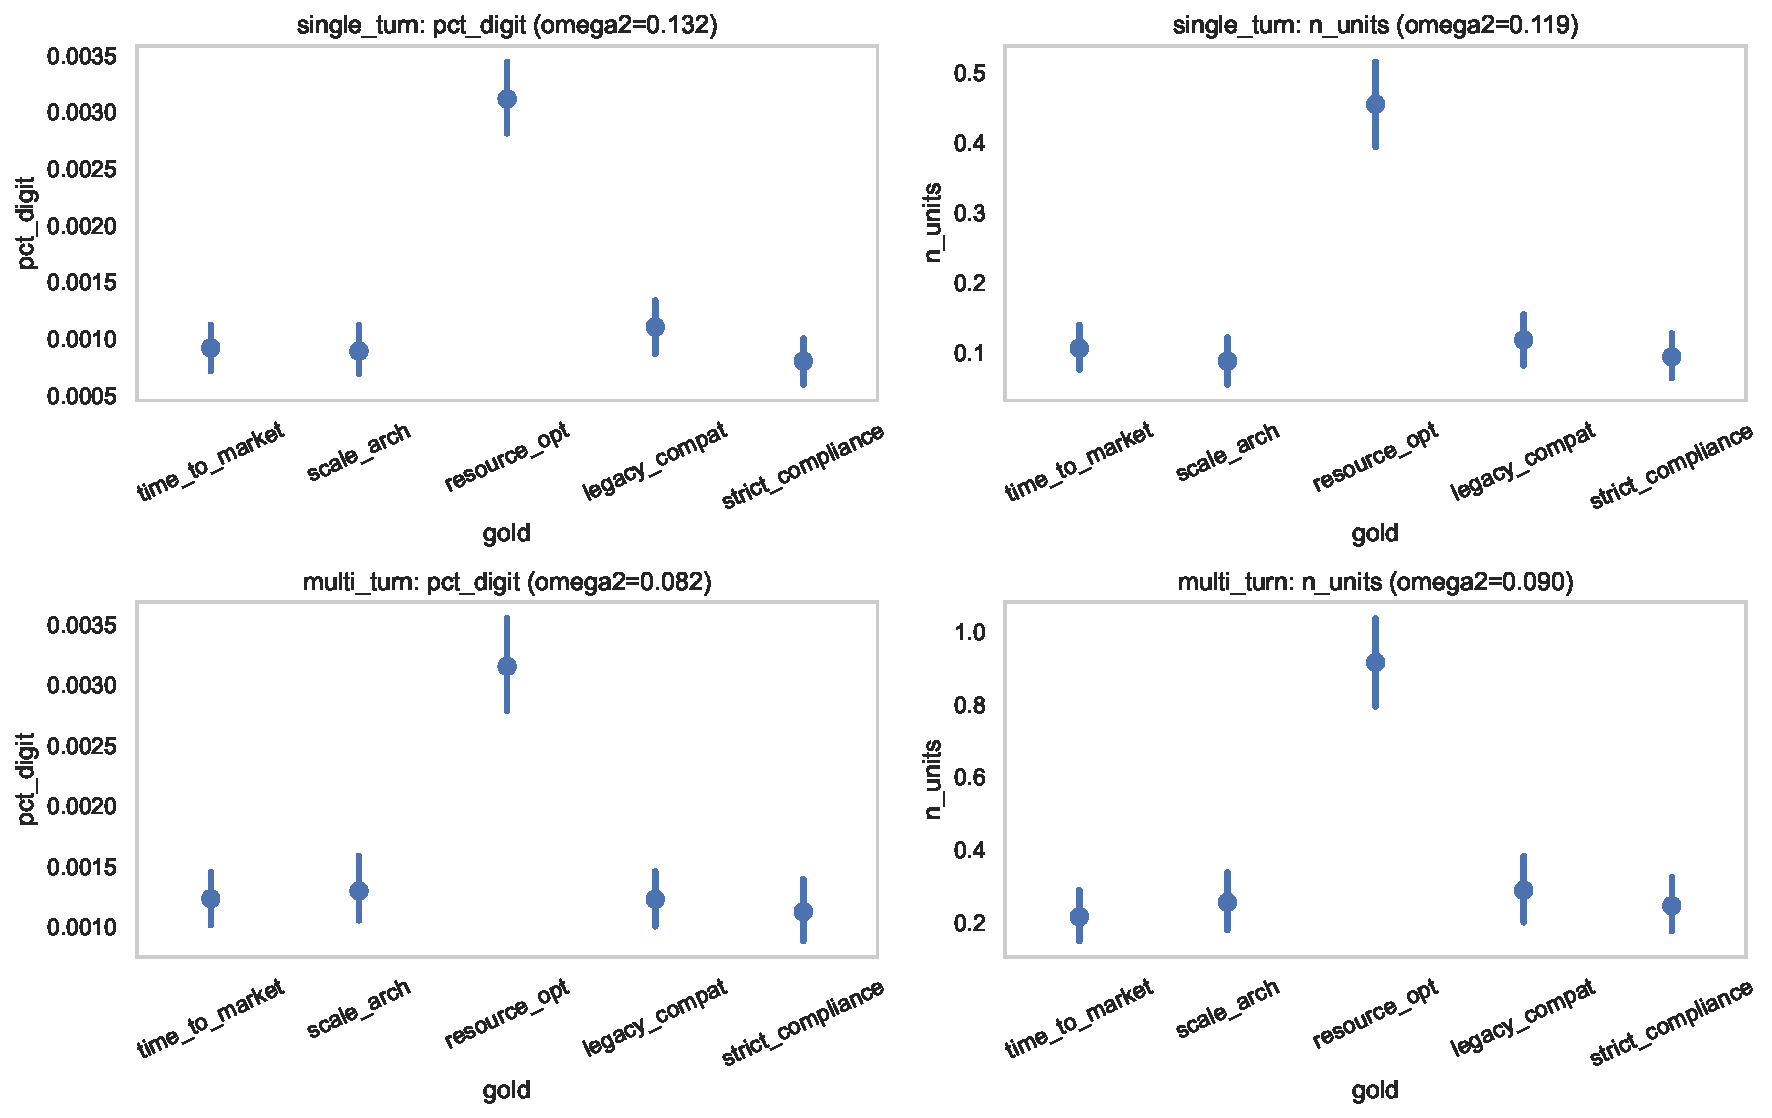
\includegraphics[width=\textwidth]{images/plots/anova/dataset_gold.pdf}
    \caption[Group means of \texttt{pct\_digit} and \texttt{n\_units} by \texttt{gold}]{Group means of \texttt{pct\_digit} and \texttt{n\_units} by \texttt{gold}, single-turn (top) and multi-turn (bottom).}
    \label{fig:gold-effect}
\end{figure}

\subsection{Levene's Test and the Kruskal-Wallis Test}
\label{subsubsec:levene-kruskal}

The one-way ANOVA in Section~\ref{subsec:anova-oneway} is valid only if the five \texttt{gold} groups share the same variance. If this assumption fails for a feature, the ANOVA's $p$-value for that feature cannot be trusted, and the effect it reports could be a product of unequal variance rather than a real difference between the groups. Two additional tests check this assumption and its consequences:

\begin{itemize}
    \item \textbf{Levene}'s test checks directly whether the five groups have equal variance, the assumption the ANOVA needs \citep{montgomeryDesignAnalysisExperiments2022}.
    \item The \textbf{Kruskal-Wallis} test \citep{montgomeryDesignAnalysisExperiments2022} compares the same \texttt{gold} groups on the ranks of the values instead of the raw values. This comparison needs no assumption about variance, so it stays valid even on a feature where Levene shows the ANOVA's assumption fails, and its verdict serves as a check on the ANOVA's own verdict for that feature.
\end{itemize}

Table~\ref{tab:levene-kruskal} reports both tests on the same thirteen features and the same \texttt{gold} factor as Table~\ref{tab:gold-omega2}, with both $p$-values corrected with Holm across that same family of thirteen tests. Bold marks a $p_{\text{holm}}$ below 0.05, rejecting the test's null hypothesis.

\begin{table}[htbp]
    \centering
    \small
    \begin{tabular}{@{}lrrrr@{}}
        \toprule
        & \multicolumn{2}{c}{\textbf{Single-turn}} & \multicolumn{2}{c}{\textbf{Multi-turn}} \\
        \textbf{Feature} & \textbf{Levene} $p_{\text{holm}}$ & \textbf{Kruskal} $p_{\text{holm}}$ & \textbf{Levene} $p_{\text{holm}}$ & \textbf{Kruskal} $p_{\text{holm}}$ \\
        \midrule
        \texttt{pct\_digit}        & \textbf{$<$0.001} & \textbf{$<$0.001} & \textbf{$<$0.001} & \textbf{$<$0.001} \\
        \texttt{n\_units}          & \textbf{$<$0.001} & \textbf{$<$0.001} & \textbf{$<$0.001} & \textbf{$<$0.001} \\
        \texttt{mean\_word\_len}   & 1.000          & \textbf{$<$0.001} & 1.000          & \textbf{$<$0.001} \\
        \texttt{long\_word\_ratio} & 0.654          & \textbf{$<$0.001} & 1.000          & \textbf{$<$0.001} \\
        \texttt{n\_comma}          & \textbf{0.002} & \textbf{$<$0.001} & 1.000          & \textbf{$<$0.001} \\
        \texttt{n\_chars}          & \textbf{0.009} & \textbf{$<$0.001} & 1.000          & \textbf{$<$0.001} \\
        \texttt{n\_words}          & \textbf{0.048} & \textbf{0.002} & 1.000          & \textbf{0.034} \\
        \texttt{n\_number\_words}  & 0.364          & \textbf{$<$0.001} & 0.555          & \textbf{0.001} \\
        \texttt{ttr}               & 0.504          & \textbf{$<$0.001} & 1.000          & \textbf{0.001} \\
        \texttt{pct\_upper}        & \textbf{$<$0.001} & \textbf{0.004} & \textbf{$<$0.001} & 0.282          \\
        \texttt{mean\_sent\_len}   & 1.000          & \textbf{0.047} & 1.000          & 1.000          \\
        \texttt{n\_sentences}      & 0.271          & 0.426          & 1.000          & 1.000          \\
        \texttt{n\_question}       & 1.000          & 0.929          & 1.000          & 1.000          \\
        \bottomrule
    \end{tabular}
    \caption[Levene and Kruskal-Wallis tests on \texttt{gold}, single-turn and multi-turn]{Levene's test and the Kruskal-Wallis test on the \texttt{gold} factor, single-turn and multi-turn.}
    \label{tab:levene-kruskal}
\end{table}

\textbf{Levene}'s test rejects equal variance on six features in the single-turn dataset (\texttt{pct\_digit}, \texttt{n\_units}, \texttt{n\_comma}, \texttt{n\_chars}, \texttt{n\_words}, \texttt{pct\_upper}) and three in the multi-turn dataset (\texttt{pct\_digit}, \texttt{n\_units}, \texttt{pct\_upper}). The ANOVA's equal-variance assumption therefore does not hold for these features.

The \textbf{Kruskal-Wallis} test reaches the same verdict as the ANOVA on twelve of the thirteen features in the single-turn dataset and on all thirteen in the multi-turn dataset. The one exception is \texttt{mean\_sent\_len} in single-turn: the ANOVA does not reject its null hypothesis ($p_{\text{holm}} = 0.120$), but the Kruskal-Wallis test does ($p_{\text{holm}} = 0.047$). This feature has the smallest effect size in Table~\ref{tab:gold-omega2} ($\omega^2 = 0.004$), and both raw $p$-values are close to 0.05 before correction ($p = 0.040$ for the ANOVA, $p = 0.016$ for Kruskal-Wallis). After Holm's correction, one is above 0.05 and the other is below it. Levene's test does not reject equal variance for this feature ($p_{\text{holm}} = 1.000$), so the disagreement is not caused by a violated assumption.

Levene's test shows that the ANOVA's equal-variance assumption fails for a minority of features, six in single-turn and three in multi-turn. Despite this, the Kruskal-Wallis test agrees with the ANOVA on every feature but one, even though it needs no such assumption. The $\omega^2$ values in Table~\ref{tab:gold-omega2} therefore describe a property of the data, not an artifact of the ANOVA's violated assumption.

\subsection{Games-Howell Test}
\label{subsec:anova-posthoc}

The one-way ANOVA does not identify which pairs of sub-agents differ on a feature. To test this, a Games-Howell test is performed on every feature whose one-way \texttt{gold} effect stays significant after the Holm correction and reaches an $\omega^2$ of at least 0.01, the conventional threshold for a small effect.

The Games-Howell test compares every pair of sub-agents on a feature, all ten pairs at once, and holds the probability of at least one false positive among them at 0.05. Unlike Tukey's HSD test \citep{montgomeryDesignAnalysisExperiments2022}, it does not assume equal variances across groups \citep{gamesPairwiseMultipleComparison1976}, so it applies directly to the features where Section~\ref{subsubsec:levene-kruskal} shows this assumption fails.
After the Games-Howell test, the $p$-values from all pairwise comparisons are corrected with Holm across the restricted family of features.

Figure~\ref{fig:posthoc} shows the pairwise mean differences for the four features with the largest \texttt{gold} effect. A blank cell marks a pair that is not significant after the Holm correction.

\begin{figure}[htbp]
    \centering
    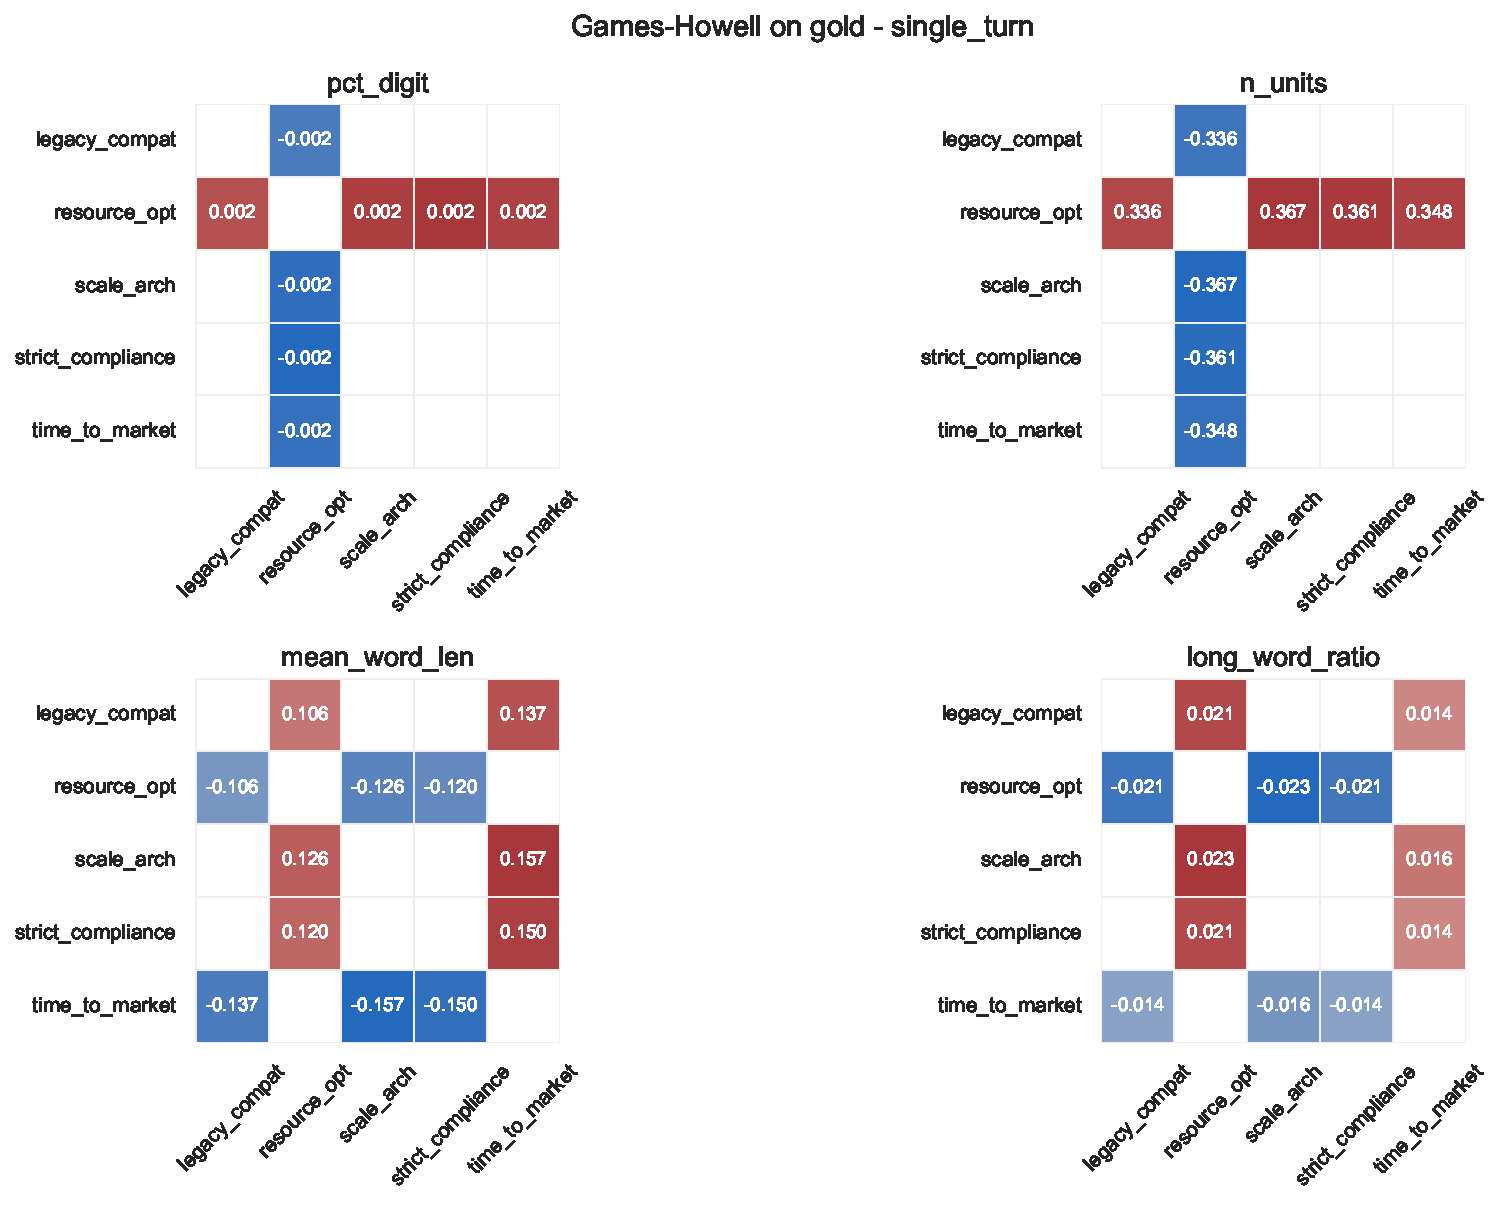
\includegraphics[width=\textwidth,height=0.46\textheight,keepaspectratio]{images/plots/anova/dataset_posthoc_single_turn.pdf}
    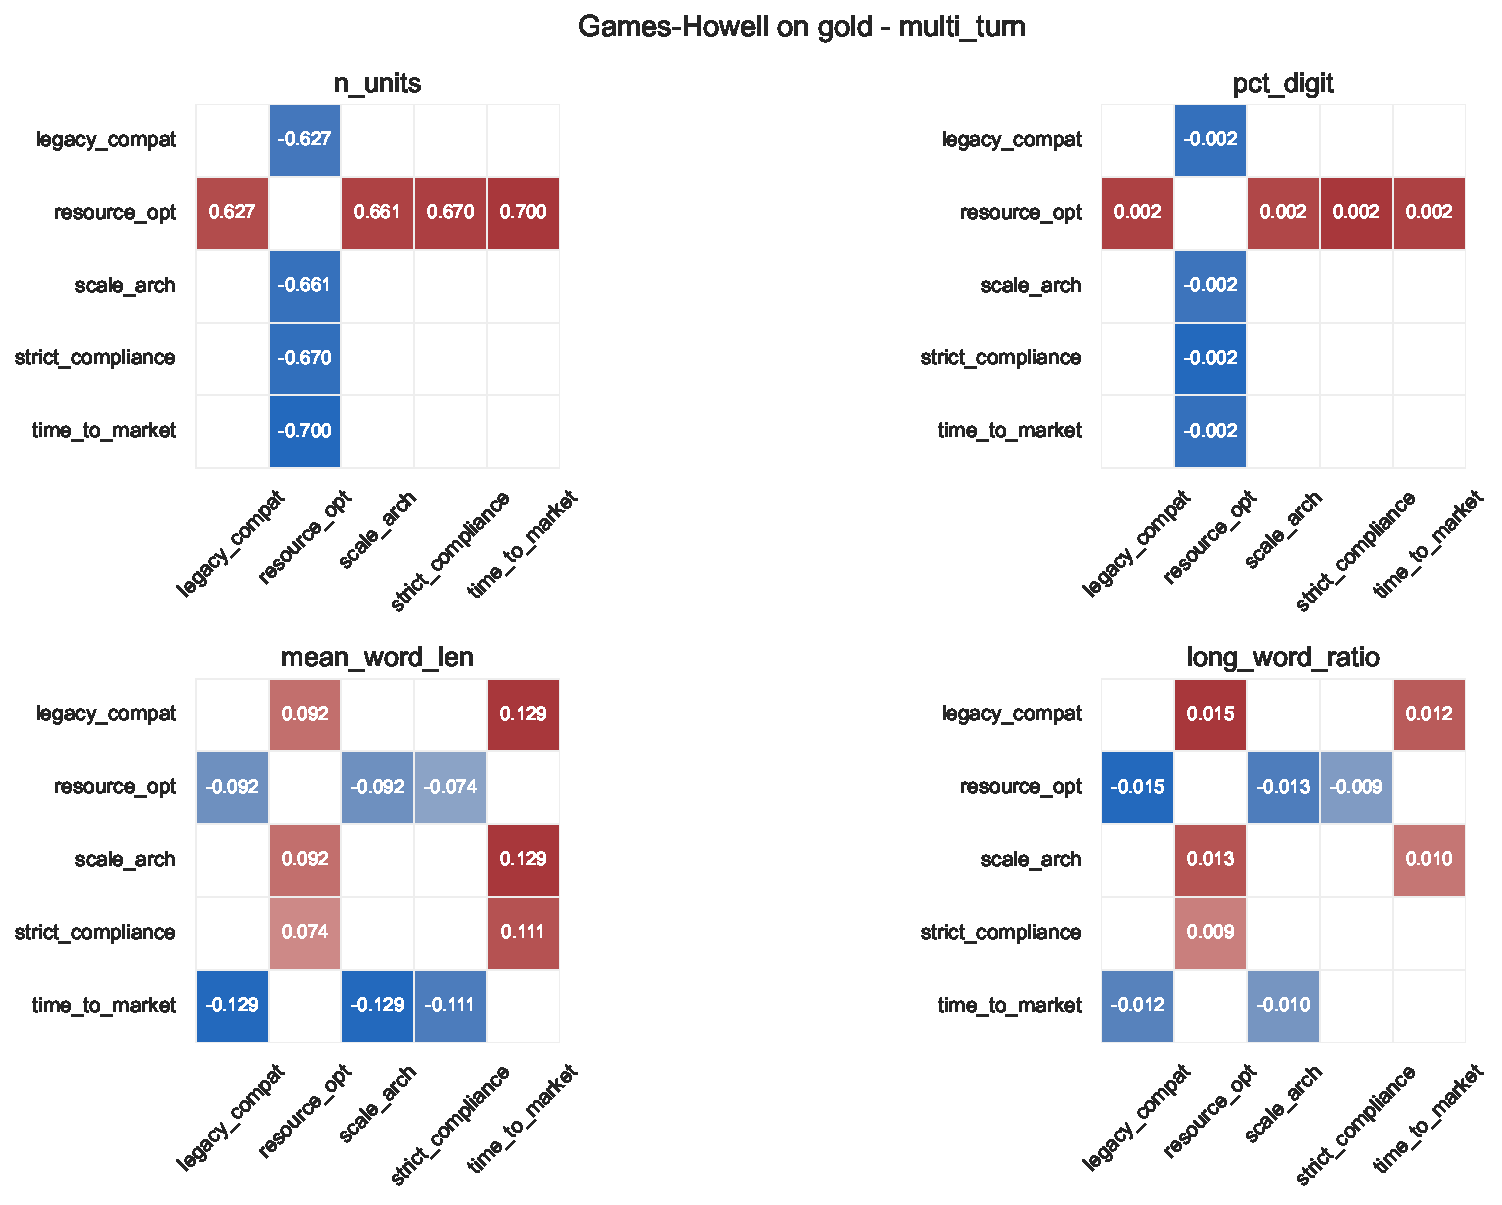
\includegraphics[width=\textwidth,height=0.46\textheight,keepaspectratio]{images/plots/anova/dataset_posthoc_multi_turn.pdf}
    \caption[Games-Howell pairwise comparisons on \texttt{gold} by dataset]{Games-Howell pairwise comparisons on \texttt{gold}, for the four surface features with the largest one-way effect, single-turn (top) and multi-turn (bottom) dataset. A blank cell means the pair is not significant after the Holm correction.}
    \label{fig:posthoc}
\end{figure}

The results on the single-turn dataset show the following structure:
\begin{itemize}
    \item On \texttt{pct\_digit} and \texttt{n\_units}, \texttt{resource\_opt} differs significantly from each of the other four sub-agents. None of the six pairs among those other four is significant. These two features therefore separate \texttt{resource\_opt} from the rest, but do not separate the remaining four sub-agents from each other.
    \item On \texttt{mean\_word\_len} and \texttt{long\_word\_ratio}, the sub-agents split into two blocks: \texttt{time\_to\_market} and \texttt{resource\_opt} on one side, \texttt{scale\_arch}, \texttt{legacy\_compat}, and \texttt{strict\_compliance} on the other. Every pair across the two blocks is significant, and no pair inside either block is. This split reflects domain-specific vocabulary: terms such as \textit{compliance}, \textit{infrastructure}, and \textit{migration} run longer than terms such as \textit{ship}, \textit{weeks}, and \textit{quick}.
\end{itemize}

The results on the multi-turn dataset show the same structure, with one exception:
\begin{itemize}
    \item On \texttt{pct\_digit} and \texttt{n\_units}, \texttt{resource\_opt} again differs significantly from each of the other four sub-agents, with no significant pair among those four.
    \item On \texttt{mean\_word\_len}, the same two blocks reappear: every pair across the two blocks is significant, and no pair inside either block is. On \texttt{long\_word\_ratio}, the same holds for five of the six pairs across the two blocks. The sixth pair, \texttt{time\_to\_market} against \texttt{strict\_compliance}, is not significant, even though the two sub-agents fall on opposite blocks.
\end{itemize}

This test confirms the same distinction among the five sub-agents. On \texttt{pct\_digit} and \texttt{n\_units}, \texttt{resource\_opt} separates from the other four. On \texttt{mean\_word\_len} and \texttt{long\_word\_ratio}, the five sub-agents split into two vocabulary blocks.

The stylistic imbalance that the one-way ANOVA detects is therefore not spread evenly across the five sub-agents. It traces to two distinct sources: \texttt{resource\_opt} stated apart from the other four by its numeric magnitude markers, and a two-block split in word length that follows domain vocabulary rather than the five sub-agents individually. Neither source separates all five sub-agents from each other on any single feature.

\subsection{Multiway ANOVA}
\label{subsec:anova-multiway}

The one-way test in Section~\ref{subsec:anova-oneway} examines one factor at a time. A \emph{multiway ANOVA} tests several factors together, so that the effect of each factor is estimated while holding the others fixed, and can also test whether two factors interact, that is, whether the effect of one factor changes depending on the level of the other. If, for example, \texttt{resource\_opt} requests used longer words only when the decoy was \texttt{time\_to\_market}, and shorter words only when the decoy was \texttt{scale\_arch}, averaging over decoys would hide the effect entirely.

Each interaction effect is isolated by comparing two nested regressions: a \texttt{full} model containing every combination of the listed factors, and a \texttt{reduced} model containing the same factors without any combination involving \texttt{gold}. The variance that the full model explains beyond the reduced model is the variance attributable to \texttt{gold}'s interactions with the other factors in that model. This gain is reported as \textbf{partial omega squared} ($\omega_p^2$): the gain divided by the variance that the reduced model left unexplained. It is corrected the same way as the one-way $\omega^2$, but for the sampling noise of the extra columns that the full model adds, on the block of interaction terms rather than on a single term \citep{olejnikGeneralizedEtaOmega2003}. Each comparison is tested with an F-test between the two nested models, Holm-corrected across the 13 features of each model.

\raggedbottom

Three such model pairs test for interactions between \texttt{gold} and the other design factors.

\begin{itemize}
    \item \textbf{Model 1 (style):} \texttt{gold * difficulty * persona}, fit on all 1650 samples.
    \item \textbf{Model 2 (difficulty):} \texttt{gold * decoy * difficulty}, fit on the 1500 samples that carry a decoy.
    \item \textbf{Model 3 (pattern):} \texttt{gold * pattern}, fit on the 900 \texttt{adversarial} samples.
\end{itemize}

Tables~\ref{tab:interactions-single} and~\ref{tab:interactions-multi} report partial $\omega^2$ and $p_{\text{holm}}$ for every feature and every model, single-turn and multi-turn. As in Table~\ref{tab:gold-omega2}, cells are shaded by magnitude, \colorbox{omegaSmall}{small}, \colorbox{omegaMedium}{medium}, \colorbox{omegaLarge}{large}, and left unshaded when negligible, using the same 0.01/0.06/0.14 thresholds \citep{cohenStatisticalPowerAnalysis2013}, and $p_{\text{holm}}$ is bold where it rejects the null hypothesis. These thresholds were defined for the one-way case, and applying them to partial omega squared can overstate the effect \citep{olejnikGeneralizedEtaOmega2003}.

Across the 78 tests spanning the three models and both datasets, only two cells reject the null hypothesis after Holm in single-turn and three in multi-turn. Their partial $\omega^2$ stays between 0.018 and 0.030 in every case, close to the small-effect threshold rather than far above it, so the conclusion holds even if the thresholds overstate the effect as described above.

The multiway analysis therefore finds no interaction effect worth reporting beyond the one-way ANOVA in Section~\ref{subsec:anova-oneway}.

\begin{table}[H]
    \centering
    \small
    \begin{tabular}{@{}lrrrrrr@{}}
        \toprule
        & \multicolumn{2}{c}{\textbf{Model 1 (style)}} & \multicolumn{2}{c}{\textbf{Model 2 (difficulty)}} & \multicolumn{2}{c}{\textbf{Model 3 (pattern)}} \\
        \textbf{Feature} & $\omega_p^2$ & $p_{\text{holm}}$ & $\omega_p^2$ & $p_{\text{holm}}$ & $\omega_p^2$ & $p_{\text{holm}}$ \\
        \midrule
        \texttt{pct\_digit}        & -0.008 & 1.000 & -0.004 & 1.000 & -0.007 & 1.000 \\
        \texttt{n\_units}          & -0.000 & 1.000 & -0.005 & 1.000 & -0.010 & 1.000 \\
        \texttt{mean\_word\_len}   & -0.005 & 1.000 & -0.005 & 1.000 & -0.005 & 1.000 \\
        \texttt{long\_word\_ratio} & -0.003 & 1.000 & -0.008 & 1.000 & -0.003 & 1.000 \\
        \texttt{n\_comma}          & -0.002 & 1.000 & 0.004  & 1.000 & -0.002 & 1.000 \\
        \texttt{n\_chars}          & -0.001 & 1.000 & -0.000 & 1.000 & -0.000 & 1.000 \\
        \texttt{n\_words}          & -0.001 & 1.000 & 0.001  & 1.000 & -0.001 & 1.000 \\
        \texttt{n\_number\_words}  & -0.006 & 1.000 & -0.004 & 1.000 & 0.003  & 1.000 \\
        \texttt{ttr}               & 0.005  & 1.000 & -0.003 & 1.000 & 0.003  & 1.000 \\
        \texttt{pct\_upper}        & \cellcolor{omegaSmall}0.022  & \textbf{0.009} & -0.011 & 1.000 & -0.004 & 1.000 \\
        \texttt{mean\_sent\_len}   & -0.006 & 1.000 & 0.008  & 0.855 & -0.004 & 1.000 \\
        \texttt{n\_sentences}      & 0.011  & 0.490 & \cellcolor{omegaSmall}0.020  & \textbf{0.007} & 0.009  & 0.808 \\
        \texttt{n\_question}       & 0.009  & 0.867 & 0.006  & 1.000 & -0.006 & 1.000 \\
        \bottomrule
    \end{tabular}
    \caption[Partial $\omega^2$ of \texttt{gold} interaction terms, single-turn dataset]{Partial $\omega^2$ ($\omega_p^2$) of the \texttt{gold} interaction terms, single-turn dataset.}
    \label{tab:interactions-single}

    \vspace{3em}

    \begin{tabular}{@{}lrrrrrr@{}}
        \toprule
        & \multicolumn{2}{c}{\textbf{Model 1 (style)}} & \multicolumn{2}{c}{\textbf{Model 2 (difficulty)}} & \multicolumn{2}{c}{\textbf{Model 3 (pattern)}} \\
        \textbf{Feature} & $\omega_p^2$ & $p_{\text{holm}}$ & $\omega_p^2$ & $p_{\text{holm}}$ & $\omega_p^2$ & $p_{\text{holm}}$ \\
        \midrule
        \texttt{pct\_digit}        & \cellcolor{omegaSmall}0.018  & \textbf{0.045} & -0.005 & 1.000 & -0.007 & 1.000 \\
        \texttt{n\_units}          & 0.004  & 0.975 & 0.002  & 1.000 & -0.004 & 1.000 \\
        \texttt{mean\_word\_len}   & 0.010  & 0.585 & 0.010  & 0.397 & -0.000 & 1.000 \\
        \texttt{long\_word\_ratio} & 0.001  & 0.975 & 0.001  & 1.000 & 0.003  & 1.000 \\
        \texttt{n\_comma}          & -0.000 & 0.975 & 0.002  & 1.000 & 0.004  & 1.000 \\
        \texttt{n\_chars}          & 0.006  & 0.975 & 0.006  & 1.000 & -0.003 & 1.000 \\
        \texttt{n\_words}          & 0.006  & 0.975 & 0.005  & 1.000 & -0.003 & 1.000 \\
        \texttt{n\_number\_words}  & 0.006  & 0.975 & 0.005  & 1.000 & 0.006  & 1.000 \\
        \texttt{ttr}               & 0.003  & 0.975 & -0.008 & 1.000 & -0.002 & 1.000 \\
        \texttt{pct\_upper}        & \cellcolor{omegaSmall}0.030  & \textbf{$<$0.001} & -0.004 & 1.000 & -0.006 & 1.000 \\
        \texttt{mean\_sent\_len}   & 0.008  & 0.786 & 0.003  & 1.000 & -0.004 & 1.000 \\
        \texttt{n\_sentences}      & 0.007  & 0.913 & 0.010  & 0.390 & -0.002 & 1.000 \\
        \texttt{n\_question}       & \cellcolor{omegaSmall}0.019  & \textbf{0.025} & -0.004 & 1.000 & -0.004 & 1.000 \\
        \bottomrule
    \end{tabular}
    \caption[Partial $\omega^2$ of \texttt{gold} interaction terms, multi-turn dataset]{Partial $\omega^2$ ($\omega_p^2$) of the \texttt{gold} interaction terms, multi-turn dataset.}
    \label{tab:interactions-multi}
\end{table}

\flushbottom

\subsection{Classifiers on Surface Features Alone}
\label{subsec:shortcut-classifiers}

The one-way and multiway ANOVA are univariate. Several small effects could still combine into one effect that a classifier exploits. A classifier that is trained on the thirteen surface features, with no access to the request text, measures the accuracy that such a combination reaches.

Two classifiers are trained, both on the same scenario-grouped 5-fold cross-validation and the same out-of-fold accuracy, broken down by difficulty tier, as the text-only classifiers of Section~\ref{sec:dataset-baselines}:

\begin{itemize}
    \item \textbf{Logistic regression}, trained five times to isolate the contribution of the numeric features to the accuracy reached from surface features alone:
    \begin{itemize}
        \item on all thirteen features, to establish the maximum accuracy attainable from surface features alone;
        \item on the feature set without \texttt{pct\_digit}, to measure how much the percentage of digit characters contributes to accuracy;
        \item on \texttt{pct\_digit} alone, to measure that feature's own contribution;
        \item on the feature set without the numeric features (\texttt{pct\_digit}, \texttt{n\_units}, \texttt{n\_number\_words}), to measure how much digit characters, unit markers, and numbers written as words together contribute to accuracy;
        \item on the numeric features alone, to measure how much they increase classification accuracy by themselves.
    \end{itemize}
    \item \textbf{Random forest}, trained once, on all thirteen features. It gives a second, non-linear ceiling, and it is the classifier used for the feature importance attribution of Section~\ref{subsec:feature-importance}.
\end{itemize}

Figures~\ref{fig:ceiling-single} and~\ref{fig:ceiling-multi} report accuracy for each of the six runs above, with chance accuracy marked for comparison.

\begin{figure}[htbp]
    \centering
    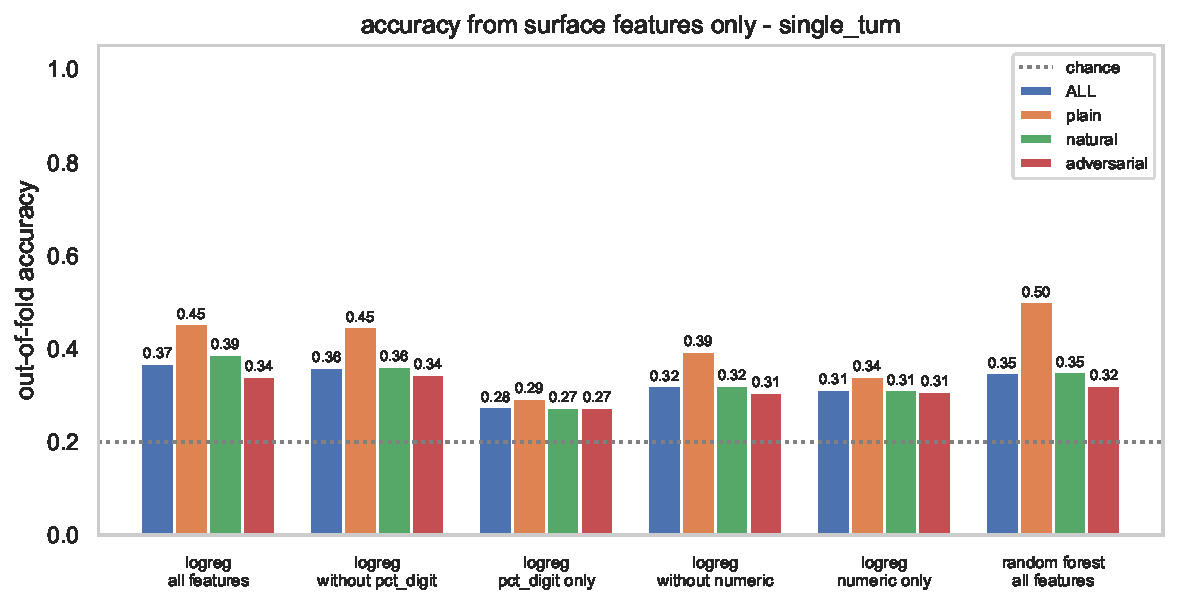
\includegraphics[width=\textwidth]{images/plots/anova/dataset_ceiling_single_turn.pdf}
    \caption[Accuracy from surface features alone, single-turn dataset]{Accuracy from surface features alone, single-turn dataset. The dotted line marks chance.}
    \label{fig:ceiling-single}
\end{figure}

\begin{figure}[htbp]
    \centering
    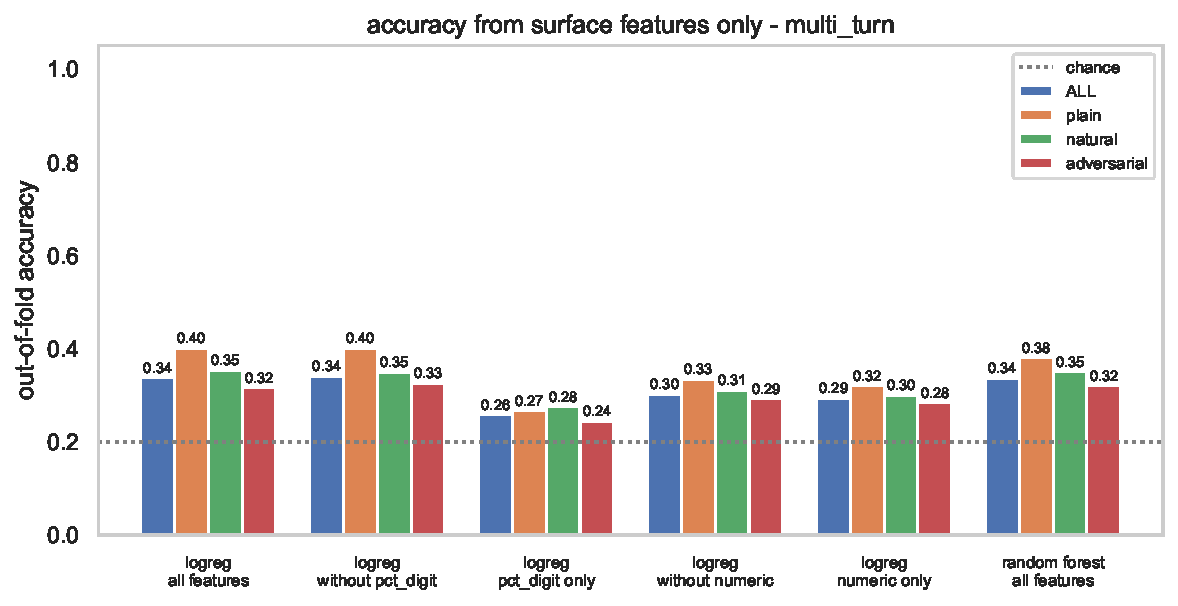
\includegraphics[width=\textwidth]{images/plots/anova/dataset_ceiling_multi_turn.pdf}
    \caption[Accuracy from surface features alone, multi-turn dataset]{Accuracy from surface features alone, multi-turn dataset. The dotted line marks chance.}
    \label{fig:ceiling-multi}
\end{figure}

Removing \texttt{pct\_digit} alone has a negligible effect on accuracy: 0.368 to 0.360 in single-turn and 0.337 to 0.341 in multi-turn. Removing all three numeric features instead costs a measurable amount of accuracy: from 0.368 to 0.320 in single-turn, and from 0.337 to 0.302 in multi-turn. The numeric features alone reach 0.313 in single-turn and 0.293 in multi-turn, nearly matching the 0.368 and 0.337 reached with all thirteen features. The other ten features therefore add only about 0.05 of accuracy beyond the numeric features. This shows that the effect of \texttt{gold} on surface features, reported in Section~\ref{subsec:anova-oneway}, is caused by the numeric features. Their accuracy alone, 0.313 and 0.293, is therefore the figure that measures the size of that effect.

Because the effect is spread across the numeric features rather than tied to \texttt{pct\_digit} alone, removing digits from the generation prompt is unlikely to lower accuracy. A magnitude such as \textit{500ms} can still be written as \textit{five hundred milliseconds}: the digit disappears, but \texttt{n\_units} or \texttt{n\_number\_words} would capture the same magnitude instead, so the information the classifier uses stays in the text. On both datasets and on every tier, the surface-only accuracy stays well below the bag-of-words baseline, 0.684 in single-turn and 0.645 in multi-turn overall, reported in Table~\ref{tab:text-baselines}. The higher accuracy that the bag-of-words classifier reaches from the request text is therefore not explained by these thirteen surface features alone.

\subsection{Feature Importance: SHAP}
\label{subsec:feature-importance}

Section~\ref{subsec:shortcut-classifiers} does not establish which of the thirteen surface features drive the accuracy of its classifiers, or which sub-agent each one favors.

\textbf{SHAP} (SHapley Additive exPlanations) \citep{lundbergUnifiedApproachInterpreting2017} assigns each feature, for a single prediction, a \emph{SHAP value}: how much that feature moved the prediction away from a baseline where no feature is known. The attribution used here, TreeSHAP \citep{lundbergExplainableAITrees2019}, requires a tree-based model, so it is computed on the random forest classifier of Section~\ref{subsec:shortcut-classifiers}, rather than on the logistic regression. Averaging the absolute SHAP value of a feature across samples ranks features by their overall contribution to the classifier. This classifier predicts one of five sub-agents, and SHAP is computed separately for each one, so a feature gets five SHAP values, one per sub-agent. A feature whose value is large for one sub-agent and small for the other four is important specifically for classifying that one sub-agent.

Figures~\ref{fig:shap-single} and~\ref{fig:shap-multi} report the mean absolute SHAP value per feature and per sub-agent, out of fold, for the seven features with the largest total, on the single-turn and the multi-turn dataset respectively.

\raggedbottom

\begin{figure}[H]
    \centering
    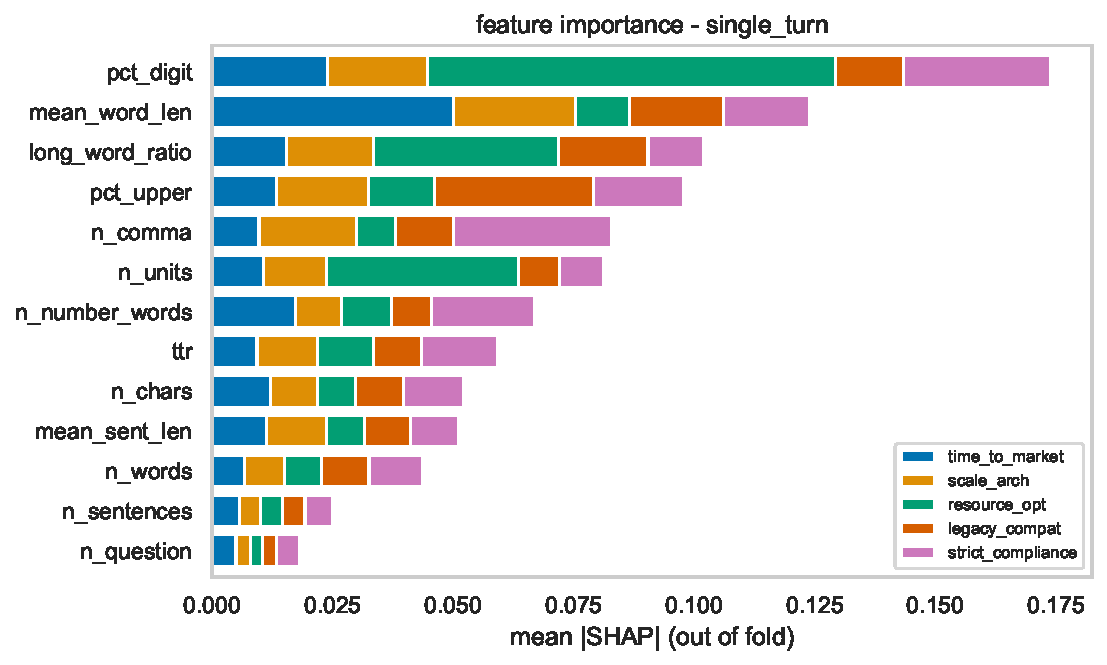
\includegraphics[width=0.9\textwidth]{images/plots/anova/dataset_shap_single_turn.pdf}
    \caption[Mean absolute SHAP value per feature and sub-agent, single-turn dataset]{Mean absolute SHAP value, out of fold, per feature and sub-agent, single-turn dataset.}
    \label{fig:shap-single}
\end{figure}

\begin{figure}[H]
    \centering
    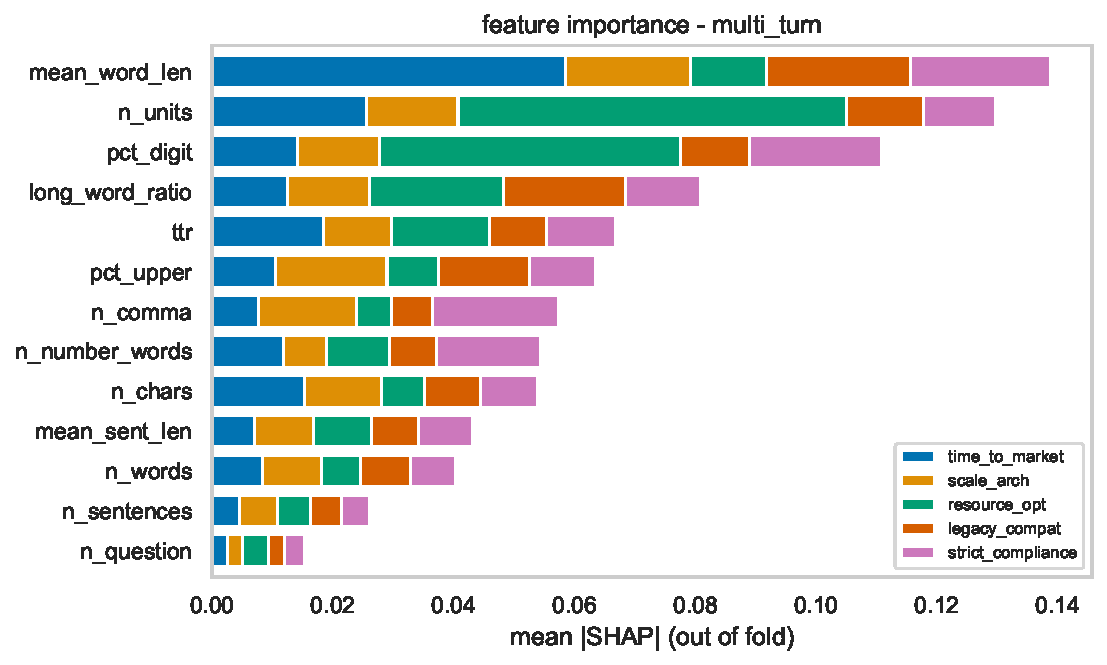
\includegraphics[width=0.9\textwidth]{images/plots/anova/dataset_shap_multi_turn.pdf}
    \caption[Mean absolute SHAP value per feature and sub-agent, multi-turn dataset]{Mean absolute SHAP value, out of fold, per feature and sub-agent, multi-turn dataset.}
    \label{fig:shap-multi}
\end{figure}

\flushbottom

Nearly half of the total SHAP attribution of \texttt{pct\_digit} concentrates on \texttt{resource\_opt} in single-turn (0.0847 of 0.174, 49\%), and the same holds for \texttt{n\_units} (49\% in both single-turn and multi-turn). This concentration is weaker for \texttt{pct\_digit} in multi-turn, at 45\%. No other feature concentrates this strongly on a single sub-agent. This confirms the Games-Howell test result of Section~\ref{subsec:anova-posthoc}. The remaining concentrations are weaker but consistent with the same test: \texttt{mean\_word\_len} concentrates on \texttt{time\_to\_market} (about 40\% in both datasets), and \texttt{n\_comma} concentrates on \texttt{strict\_compliance}.

\subsection{Summary}
\label{subsec:anova-summary}

The one-way ANOVA finds a medium effect of \texttt{gold} on only two of the thirteen surface features, \texttt{pct\_digit} and \texttt{n\_units}, both tied to numeric magnitudes in the request text. Every other feature reaches at most a small effect. The Games-Howell test and the SHAP attribution trace the effect on \texttt{pct\_digit} and \texttt{n\_units} to a single sub-agent: \texttt{resource\_opt} states memory ceilings, cost budgets, and latency figures more often than the other four sub-agents, and \texttt{pct\_digit} and \texttt{n\_units} do not separate those other four sub-agents from each other. The multiway ANOVA finds the \texttt{gold} effect on \texttt{pct\_digit} and \texttt{n\_units} independent of \texttt{difficulty}, \texttt{persona}, \texttt{decoy}, and \texttt{pattern}: almost all interaction tests fail to reject the null hypothesis.

Section~\ref{subsec:lexical-separability} requires the sub-agents to be balanced in writing style, not only in vocabulary, and the analysis in this section shows this requirement is not met exactly: \texttt{pct\_digit}, \texttt{n\_units}, \texttt{mean\_word\_len}, and \texttt{long\_word\_ratio} all differ significantly across \texttt{gold}. The purpose of that requirement is to keep a text-only classifier from routing a request by a stylistic marker instead of by its content. A classifier trained on the thirteen surface features reaches its ceiling accuracy almost entirely from the numeric features alone, 0.313 in single-turn and 0.293 in multi-turn against 0.368 and 0.337 for the full feature set (Section~\ref{subsec:shortcut-classifiers}). Both figures stay well below the bag-of-words baseline of 0.684 and 0.645 (Table~\ref{tab:text-baselines}).

Since the thirteen surface features cannot reach that baseline, the accuracy of the bag-of-words classifier must come from the lexical content of the request, the word choices the surface features do not capture, rather than from its style. Besides the numeric features, only \texttt{mean\_word\_len} and \texttt{long\_word\_ratio} differ significantly across \texttt{gold}, and they add only about 0.05 of accuracy over the numeric features alone (Section~\ref{subsec:shortcut-classifiers}). This residual style imbalance is too small for a text-only classifier to route requests by style at a level that would compromise the purpose of the balance requirement in Section~\ref{subsec:lexical-separability}: keeping a request from being routed by how it is written instead of what it asks.

